\documentclass{article}
\usepackage{amsmath}
\usepackage{geometry}
\usepackage{float}
\geometry{a4paper, left=2cm, right=2cm, top=2.54cm, bottom=2.54cm}
\usepackage{indentfirst}
\usepackage{enumitem}
\usepackage{bm}
\usepackage[hidelinks]{hyperref}

% 段落間距  (begin doc 才設定)
\usepackage{parskip}
    % 普通文字,行距
    \usepackage[onehalfspacing]{setspace}
    
\usepackage{tabularx}

\usepackage{fontspec,xltxtra,xunicode}

\usepackage{titlesec}

\def\Large{\fontsize{18}{10}\selectfont}
\def\huge{\fontsize{26}{10}\selectfont}
\def\Huge{\fontsize{36}{30}\selectfont}

\titleformat{\section}
  {\fontsize{16pt}{15}\bfseries}
  {\selectfont\thesection.}
  {0.5em}
  {}

\titleformat{\subsection}
  {\fontsize{14pt}{15}\bfseries}
  {\selectfont\thesection.}
  {0.5em}
  {}


\usepackage{xeCJK}
\setCJKmainfont[AutoFakeBold=3]{DFKai-SB} %设置中文字体\XeTeXlinebreaklocale “zh”\XeTeXlinebreakskip = 0pt plus 1pt minus 0.1pt %文章内中文自动换行


\usepackage{minted}
\setminted{
baselinestretch=1,
fontsize=\small,
python3=true,
style = tango,
}


\usepackage{caption}
\newenvironment{code}{\captionsetup{type=listing, font=large}}{}

\captionsetup{font=large}



\usepackage{longtable}
\usepackage{array}
\usepackage{makecell}
\renewcommand{\arraystretch}{1.2}

% % 首行縮排
% \usepackage{indentfirst}
% % 首行縮排距離
% \setlength\parindent{28pt}

\renewcommand{\figurename}{Fig.}

\setmainfont{Times New Roman}

\title{\textbf{{\huge HW5} \\ 記憶體積體電路\ Memory\ Circuit\ Design}}
\author{{\Large\textbf{ 電機4A\quad 109501201\quad 陳緯亭}}}
\date{\Large{\today}} 



\begin{document}

% 首行縮排距離
\setlength\parindent{28pt}

% 段落後間距
\setlength\parskip{14pt}



\newcolumntype{L}[1]{>{\raggedright\let\newline\\\arraybackslash\hspace{0pt}}m{#1}}
\newcolumntype{C}[1]{>{\centering\let\newline\\\arraybackslash\hspace{0pt}}m{#1}}
\newcolumntype{R}[1]{>{\raggedleft\let\newline\\\arraybackslash\hspace{0pt}}m{#1}}


\maketitle
\vspace*{-0.5cm}

\fontsize{12pt}{1.5em}

\selectfont



\section{Read Operation}

\subsection*{Step 1: Prechare}

打開 EQ。Bitline 和 $\rm{\overline{Bitline}}$ 穩定在參考點 $V_{ref}=\dfrac{V_{CC}}{2}$


\begin{figure}[H]
\centering
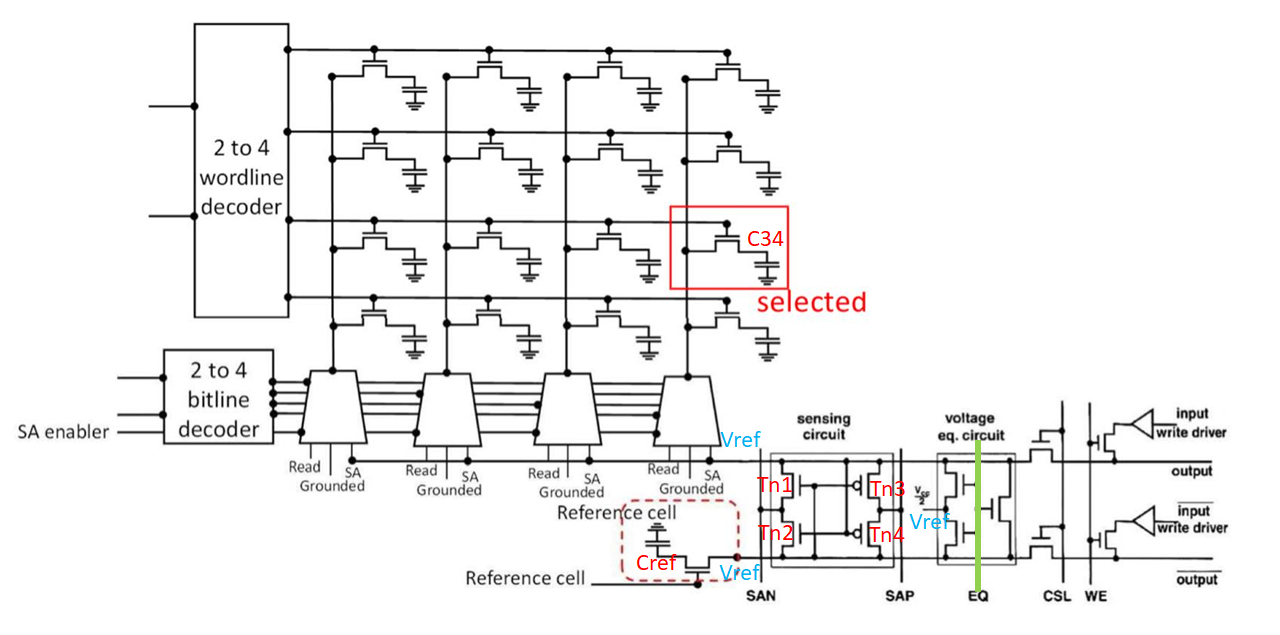
\includegraphics[width = 1\linewidth]{./img/2023-12-24-16-24-45.png}
\end{figure}

\subsection*{Step 2: Access}

關閉 EQ。開啟 Wordline。Capacitor (C34) 儲存正電荷會流向 Bitline , Capacitor (Cref) 儲存的正電荷會流向  $\rm{\overline{Bitline}}$ 。 Capacitor 有儲存正電荷的,會把 Bitline (或 $\rm{\overline{Bitline}}$ ) 的電壓拉升到 $V_{ref}+$。

\begin{figure}[H]
  \centering
  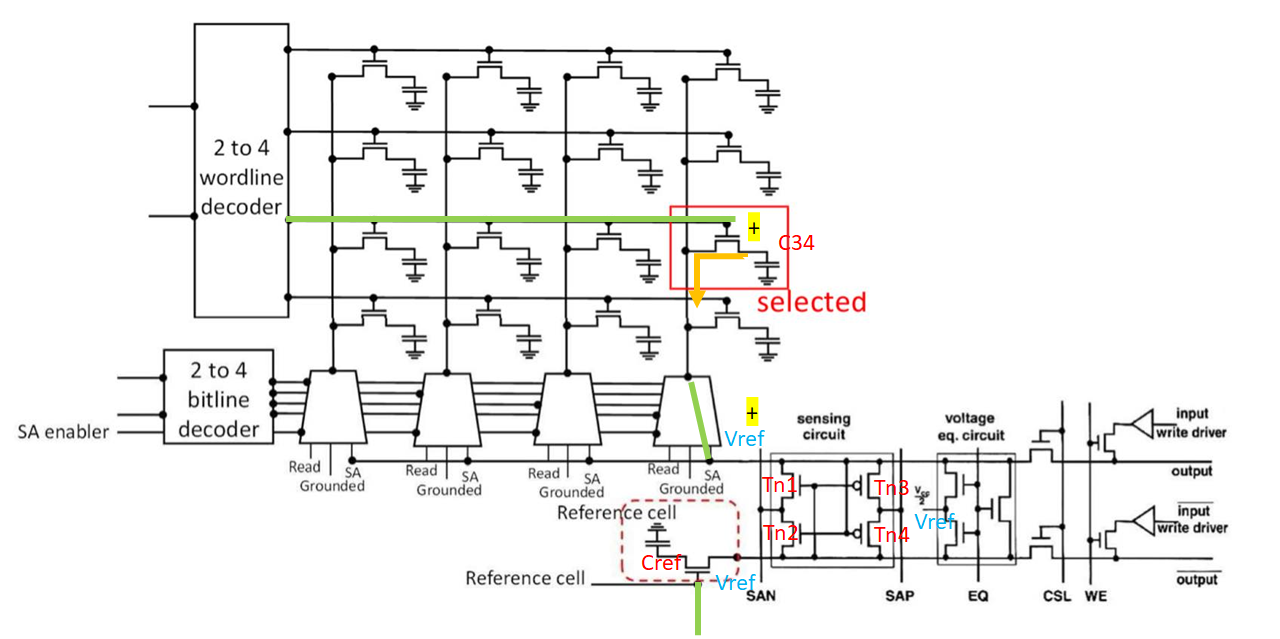
\includegraphics[width =\linewidth]{./img/2023-12-24-16-27-36.png}
  \end{figure}

\subsection*{Step 3: Sense}

如果Bitline ($\rm\overline{Bitline}$)被拉升到$V_{ref}+$。
Tn2 (Tn1) 比 Tn1 (Tn2) 更具導通性,而 Tp1 (Tp2) 比 Tp2 (Tp1) 更具導通性。
這時,SAN (Sense-Amplifier N-Fet Control) 為邏輯 0 ,SAP (Sense-Amplifier P-Fet Control) 則為邏輯 1 的電壓亦即 Vcc。藉此,$\rm\overline{Bitline}$ 上的電壓更快被 SAN 拉到 0 (1),同理,Bitline 上的電壓也被 SAP 拉到邏輯 1 (0)。 最後的穩定狀態極為儲存 Capacitor 的信息。反之亦然。

\begin{figure}[H]
  \centering
  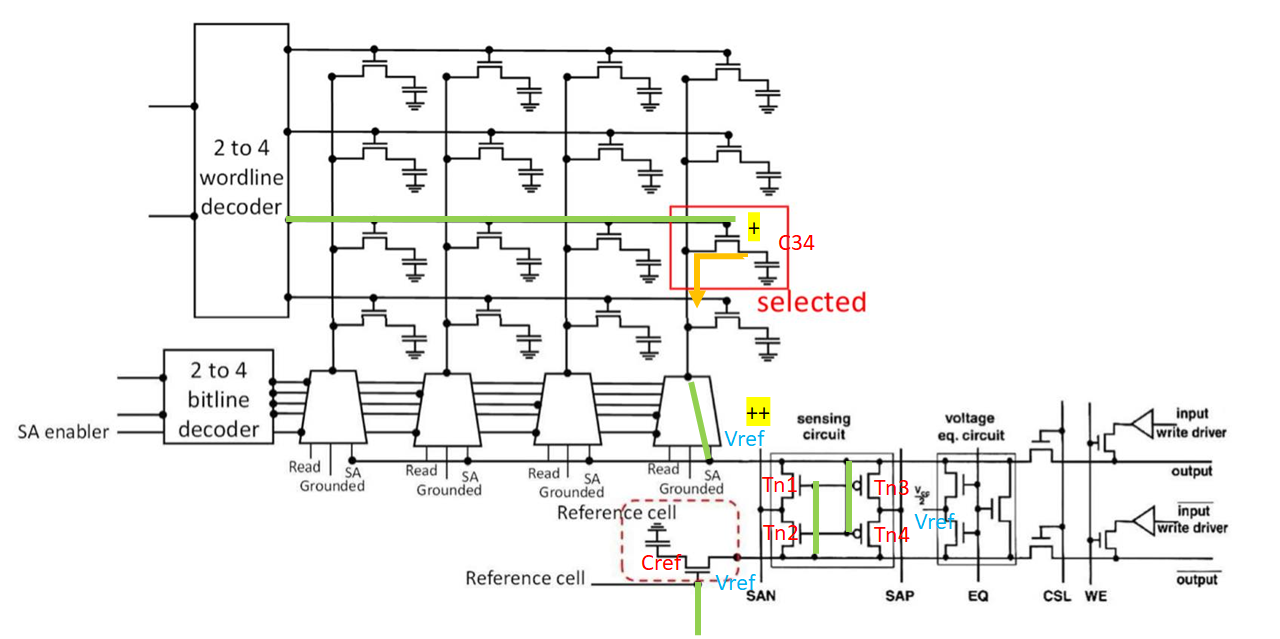
\includegraphics[width = \linewidth]{./img/2023-12-24-16-29-34.png}
  \end{figure}



\subsection*{Step 4: Restore}

Bitline 會處於的邏輯 1 (0),這時候 Bitline 會對 Capacitor 充電。經過特定時間後,Storage Capacitor 就可以恢復到Read前的狀態。
CSL 打開,外界可以從 output 和 $\rm\overline{output}$ 上Read。

\begin{figure}[H]
\centering
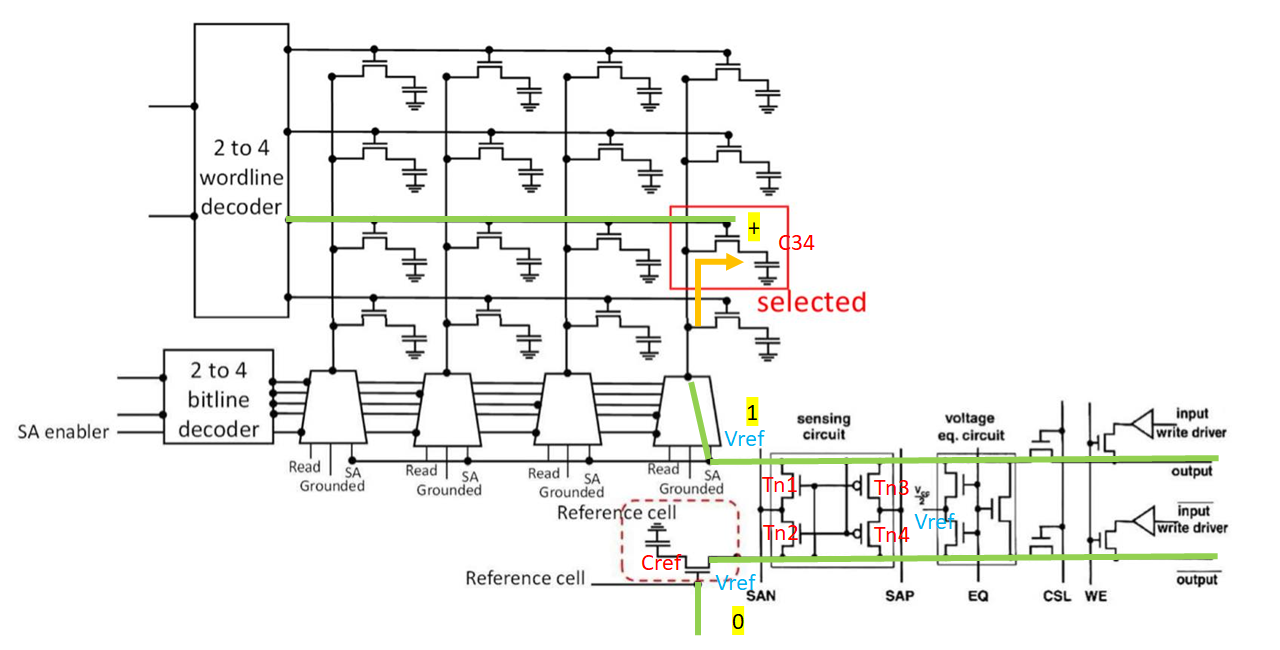
\includegraphics[width = \linewidth]{./img/2023-12-24-16-31-40.png}
\end{figure}

\section{Write Operation}

打開 WE (Write Enable)。 打開 CSL 。 打開 Wordline (WL)。此時, Bitline 會被 input 拉到 1(0) ,$\rm\overline{Bitline}$ 則被拉到邏輯 0(1)。
經過特定的時間後,即可寫入資訊到 C34  為邏輯 1(0) 和 Cref 為邏輯 0(1)。

\begin{figure}[H]
  \centering
  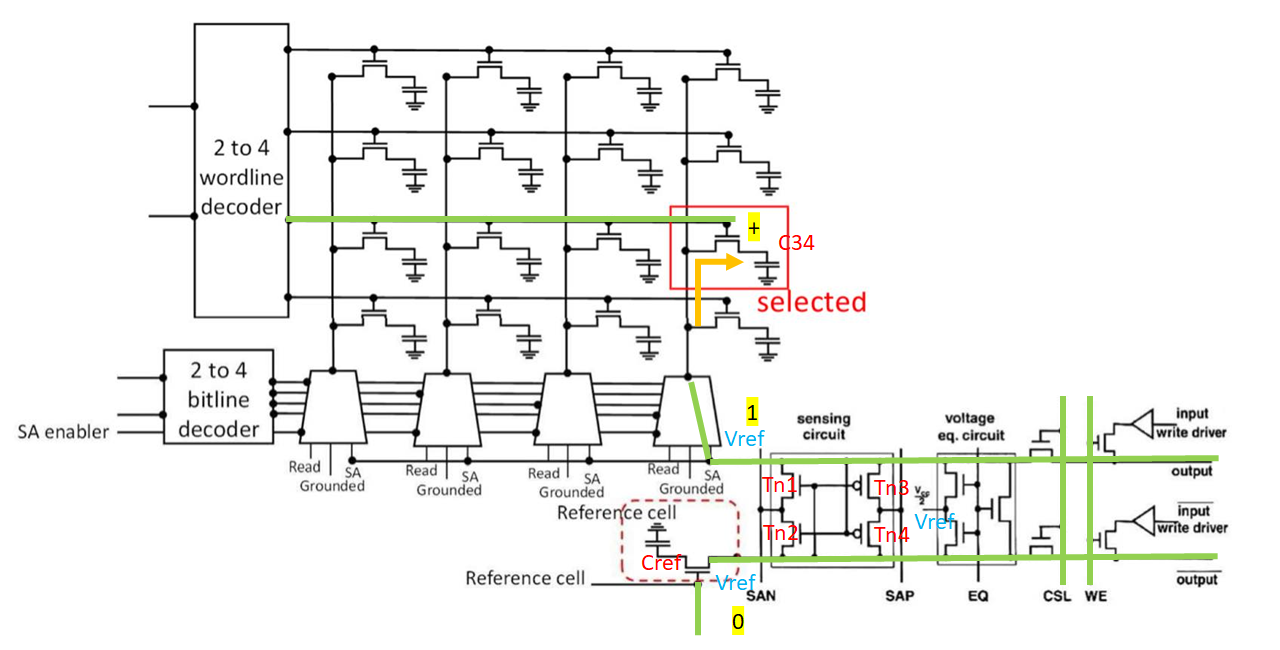
\includegraphics[width = 0.95\linewidth]{./img/2023-12-24-16-33-47.png}
  \end{figure}


\section{2 to 4 Decoder Circuit}

用兩個 2 to 4 decoder 去選擇 selected cell。wordline decoder 選擇的是 row,bitline decoder 選擇的是 colume。下圖畫的是沒有 SA enabler,有 enabler 的,只是在這 4 個 AND Gates 上各加上一個 enable input。

\begin{figure}[H]
  \centering
  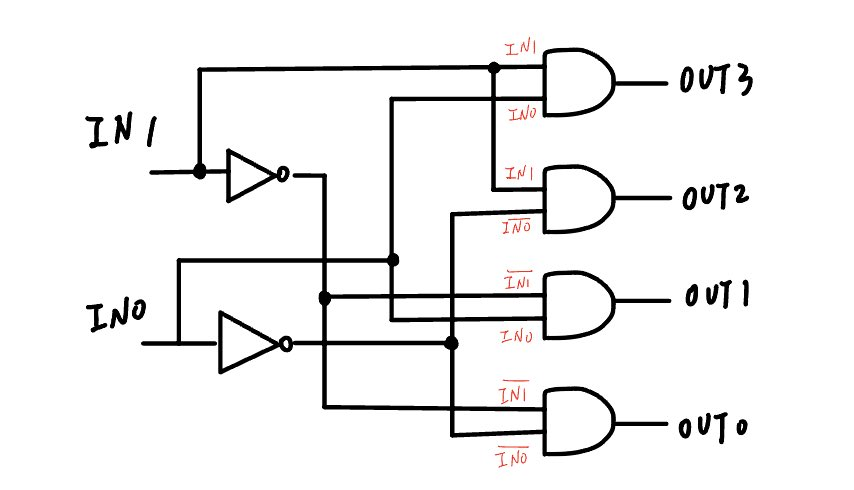
\includegraphics[width = 0.5\linewidth]{./img/2023-12-24-16-36-59.png}
  \end{figure}

\section{The SA Circuit}

用 Transmission gate 做開關 bitline decoder 選擇的 column 決定哪一個 Transmission gate 開啟接出去到 Bitline 上。在此 4x4 mini 1T1C DRAM array 會有 4 個 SA Circuit,因為有 4 個 column。

\begin{figure}[H]
  \centering
  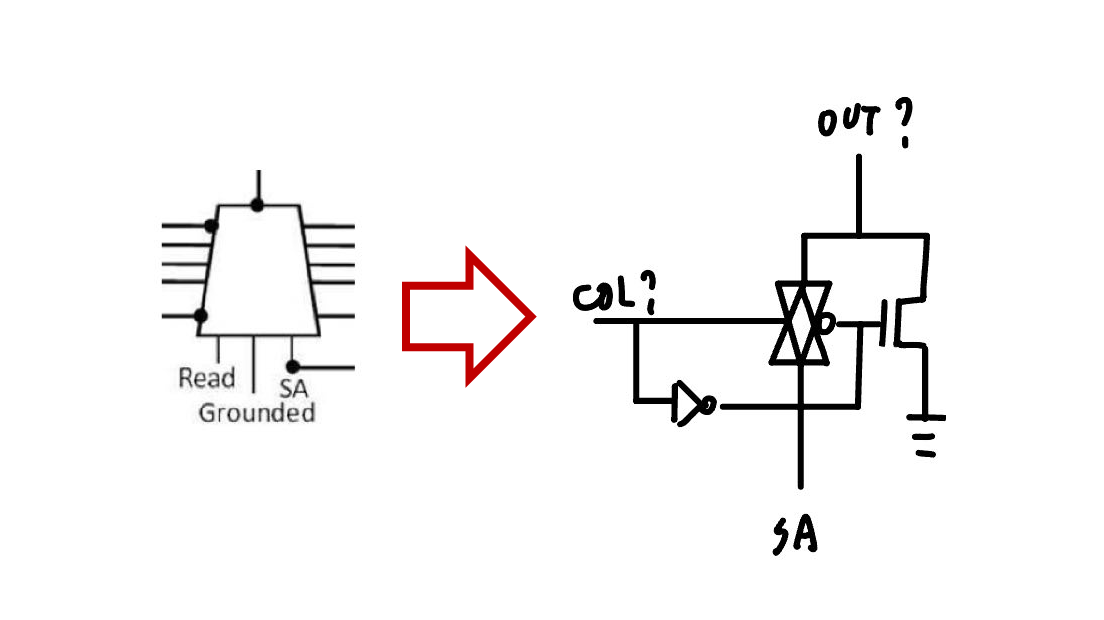
\includegraphics[width = 0.6\linewidth]{./img/2023-12-24-16-48-34.png}
  \end{figure}

  \section{參考資料}

  \begin{enumerate}
  
  \item\href{https://blog.csdn.net/highman110/article/details/131242849}{【DRAM存储器二】Sense Amplifier}
  \item\href{http://www.wowotech.net/basic_tech/307.html}{DRAM 原理 1 :DRAM Storage Cell}


\clearpage
\section{Timing}

先 Write 1、 Read 1,再來 Write 0、 Read 0。\\
圖上的 1, 2, 3, 4 操作分別為
1.	Precharge。
2.	Access。
3.	Sense。
4.	Restore。


\begin{figure}[H]
  \centering
  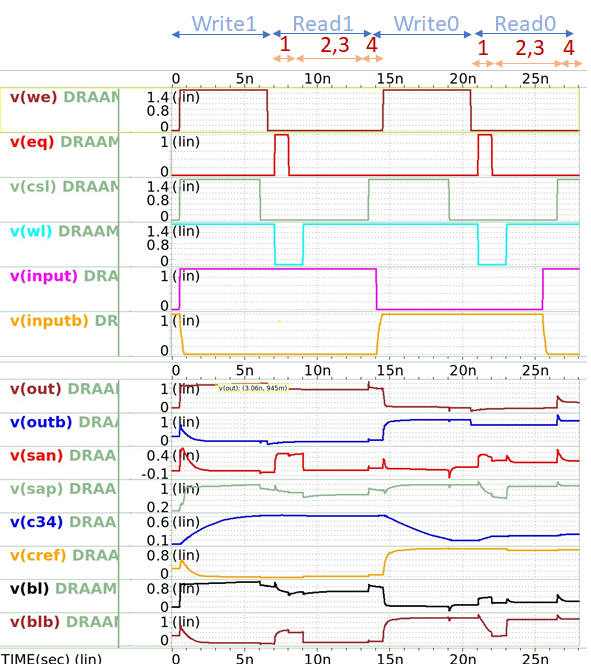
\includegraphics[width = \linewidth]{./img/2023-12-24-17-13-43.png}
  \caption{The Waveforms for Main Signal}
  \end{figure}

  \clearpage
  有設定每個 cell 的初始值,一開始的偏壓會依照初始值,unselected cell 會隨時間會有些微掉電壓或上升電壓,但不至於影響判斷結果。

  \begin{figure}[H]
  \centering
  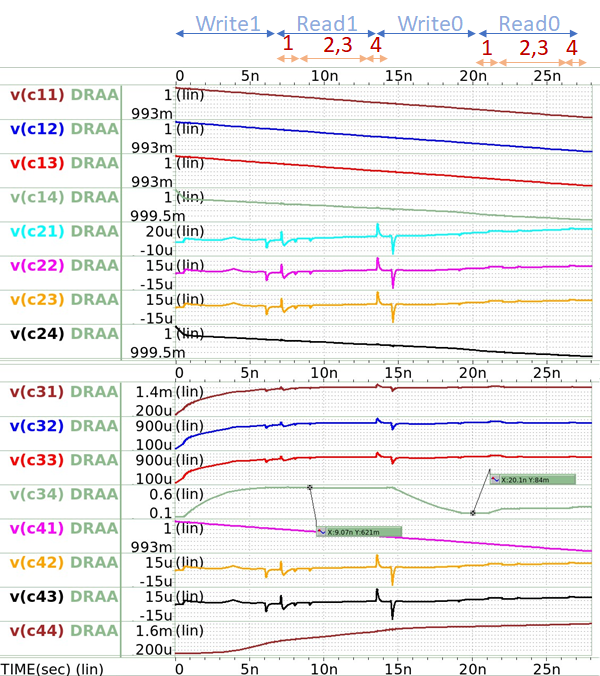
\includegraphics[width = \linewidth]{./img/2023-12-24-17-15-46.png}
  \caption{The Waveforms for each cell}
  \end{figure}


    \clearpage

    Decoder 的訊號線選擇,因為是 Select the cell at the 4th column and 3rd row (C34), 所以 ir1 = 1、ir0 = 0 選擇第 3 個 row, ic1 = 1、ic0 = 1,選擇第四個 column。SA enabler 訊號跟著 WL 的波形行動即可。

    \begin{figure}[H]
      \centering
      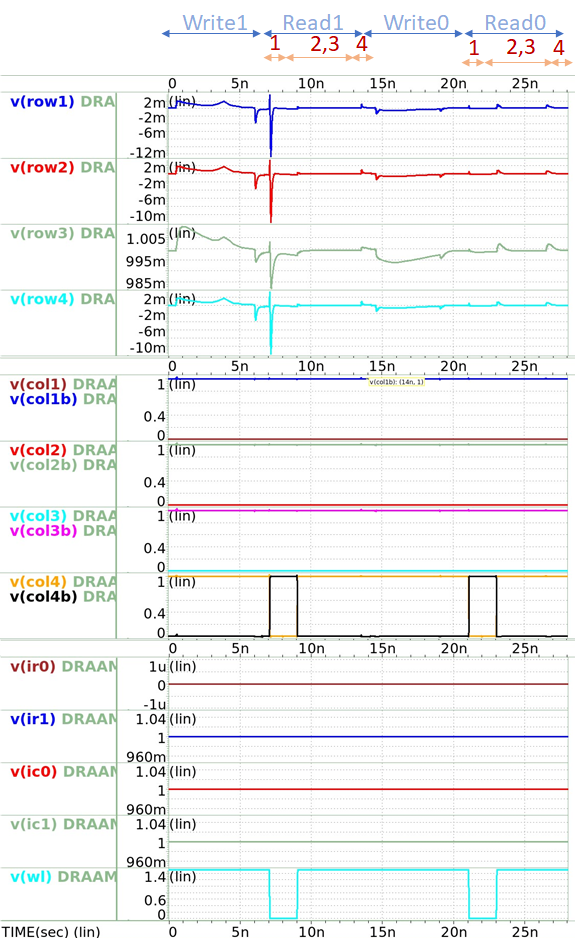
\includegraphics[width = 0.78\linewidth]{./img/2023-12-24-17-23-56.png}
      \caption{The Waveforms for Decoder Selection}
      \end{figure}
  

      \clearpage

  選擇 column 4。所以只有 out4 有電壓。

  \begin{figure}[H]
    \centering
    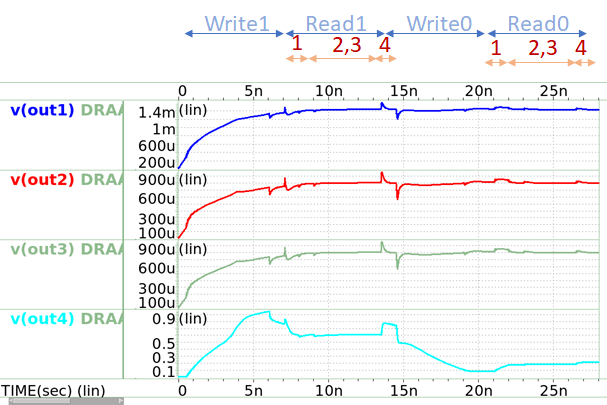
\includegraphics[width = \linewidth]{./img/2023-12-24-17-21-08.png}
    \caption{The Waveforms for Selected Column}
    \end{figure}
  

\end{enumerate}

\end{document}